\section{Error Analysis}
\label{sec:errors}
\subsection{Performance by class}
The overall scores conceal substantial variation among categories.
Figure~\ref{fig:class_f1} compares the per-class F1 values of all five models.
The full numerical table is included in Appendix~A.

\begin{figure}[H]\centering
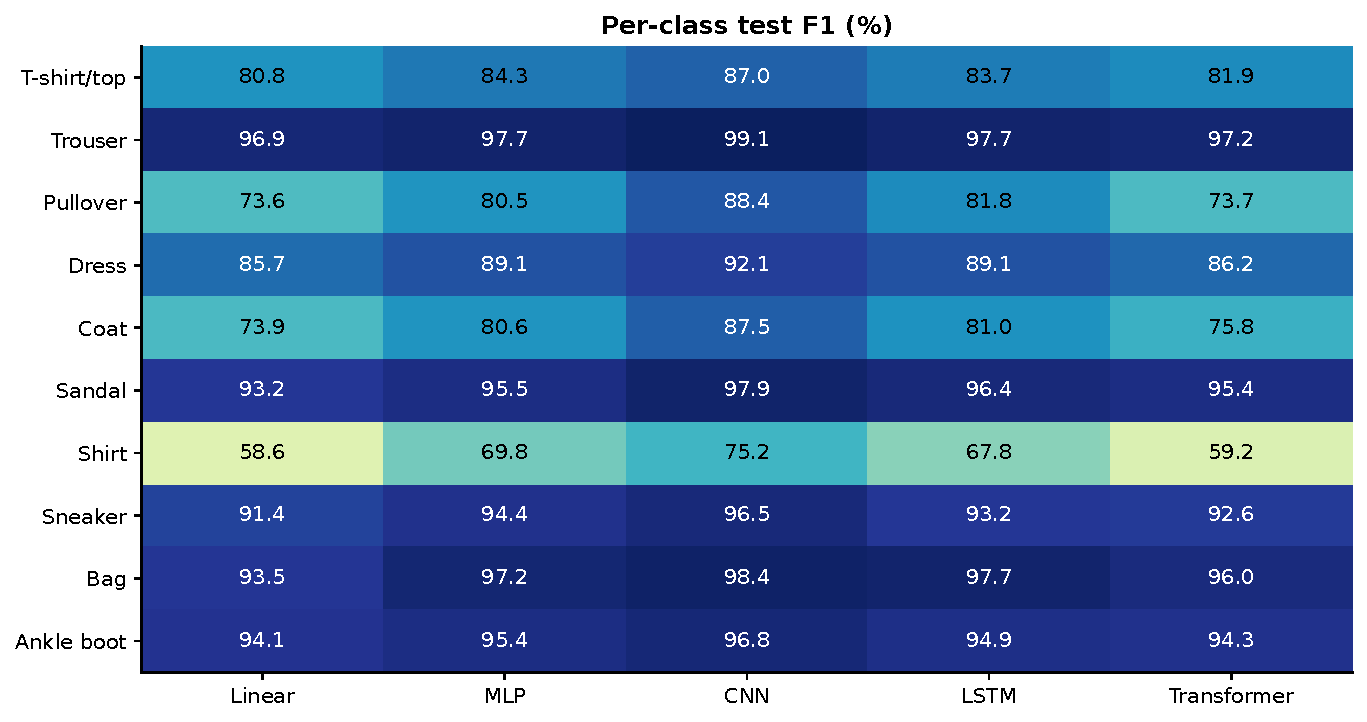
\includegraphics[width=.96\linewidth]{class_f1.pdf}
\caption{Per-class F1 on the official test set, shown as percentages.
Every class has 1,000 test images.}\label{fig:class_f1}
\end{figure}

Shirt has the lowest F1 for every model. Its score rises from 58.59\% for Linear
to 69.76\% for MLP and 75.18\% for CNN. Transformer reaches 59.20\%, which is
close to Linear on this class despite its higher overall score.

CNN has the highest F1 for each of the ten classes in the recorded runs.
Its improvement over MLP is particularly clear for Pullover
(80.54\% to 88.43\%) and Coat (80.65\% to 87.45\%).
For Trouser, both models already perform well, so the gain is smaller.

The LSTM's aggregate result is close to the MLP's, but it has higher F1 on
Pullover, Coat, Sandal and Bag, and lower F1 on Shirt and Sneaker.
For example, LSTM obtains 96.40\% F1 on Sandal versus 95.50\% for MLP,
but 67.84\% on Shirt versus 69.76\%.
The near tie in accuracy therefore does not mean the two models make the same
decisions.

These results broadly agree with the visual observations in Section~2:
upper-body categories are difficult to separate, while trousers and several
accessory or footwear categories are easier. However, class-average similarity
is only a descriptive summary. Models predict individual images, whose shapes
and textures can differ substantially from the average.

\clearpage
\subsection{Confusion patterns in the CNN}
Figure~\ref{fig:cnn_confusion} shows the CNN's confusion matrix. Rows are true
labels and columns are predicted labels. Each row contains 1,000 images.

\begin{figure}[H]\centering
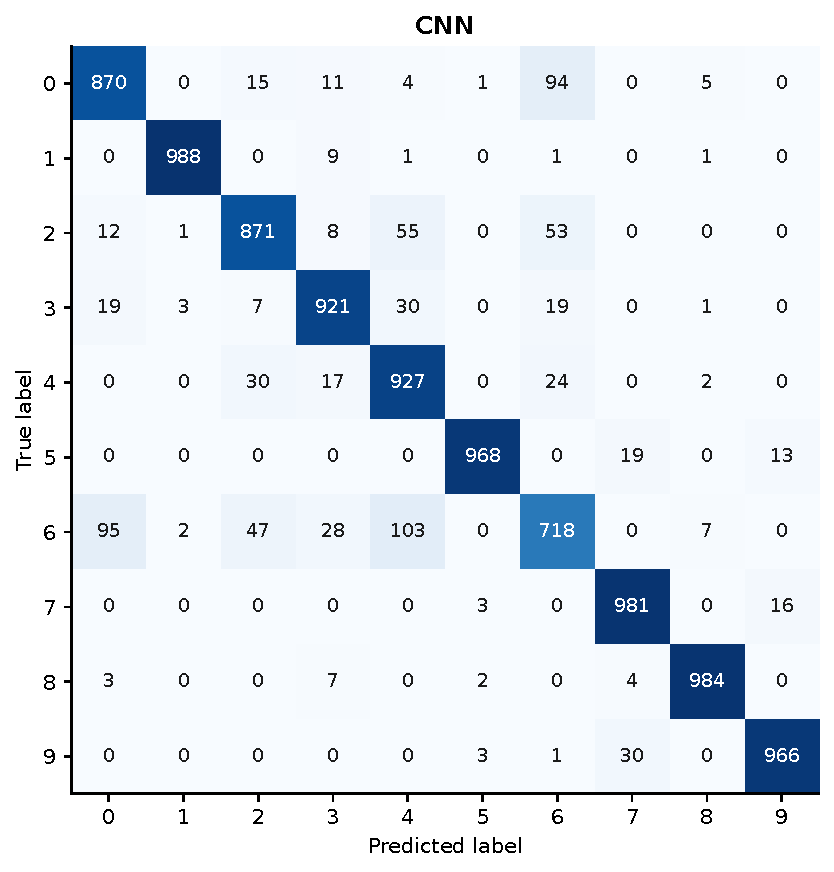
\includegraphics[width=.63\linewidth]{cnn_confusion.pdf}
\caption{CNN test confusion counts. Label IDs follow Table~\ref{tab:labels}.
The diagonal contains correct predictions.}\label{fig:cnn_confusion}
\end{figure}

\begin{table}[H]\centering
\caption{Six CNN class pairs with the largest combined two-way confusion.
The two directions are counted separately.}\label{tab:confusion_pairs}
\begin{tabular}{llrr}\toprule
Class A & Class B & A predicted as B & B predicted as A\\\midrule
\tabledata{generated/confusion_rows.tex}
\bottomrule\end{tabular}
\end{table}

Of the CNN's 806 mistakes, \UpperErrors{} occur between the four labels
T-shirt/top, Pullover, Coat and Shirt. These account for
\UpperErrorPercent\% of all errors. Shirt alone has 282 incorrect predictions:
103 become Coat, 95 become T-shirt/top and 47 become Pullover.

The confusions are not always symmetric. There are 103 Shirt-to-Coat errors
but only 24 Coat-to-Shirt errors. CNN recalls 92.7\% of Coat images, yet its
Coat precision is lower, at 82.77\%, because other garments are also predicted
as Coat. This distinction explains why recall alone would give an incomplete
view of the class.

\clearpage
\subsection{Individual predictions and shared errors}
Figure~\ref{fig:examples} displays four correct and four incorrect CNN
predictions. A seeded generator selects from the correct set and then the
incorrect set. The deliberately balanced display illustrates behavior; it
does not represent the model's actual error frequency.

\begin{figure}[H]\centering
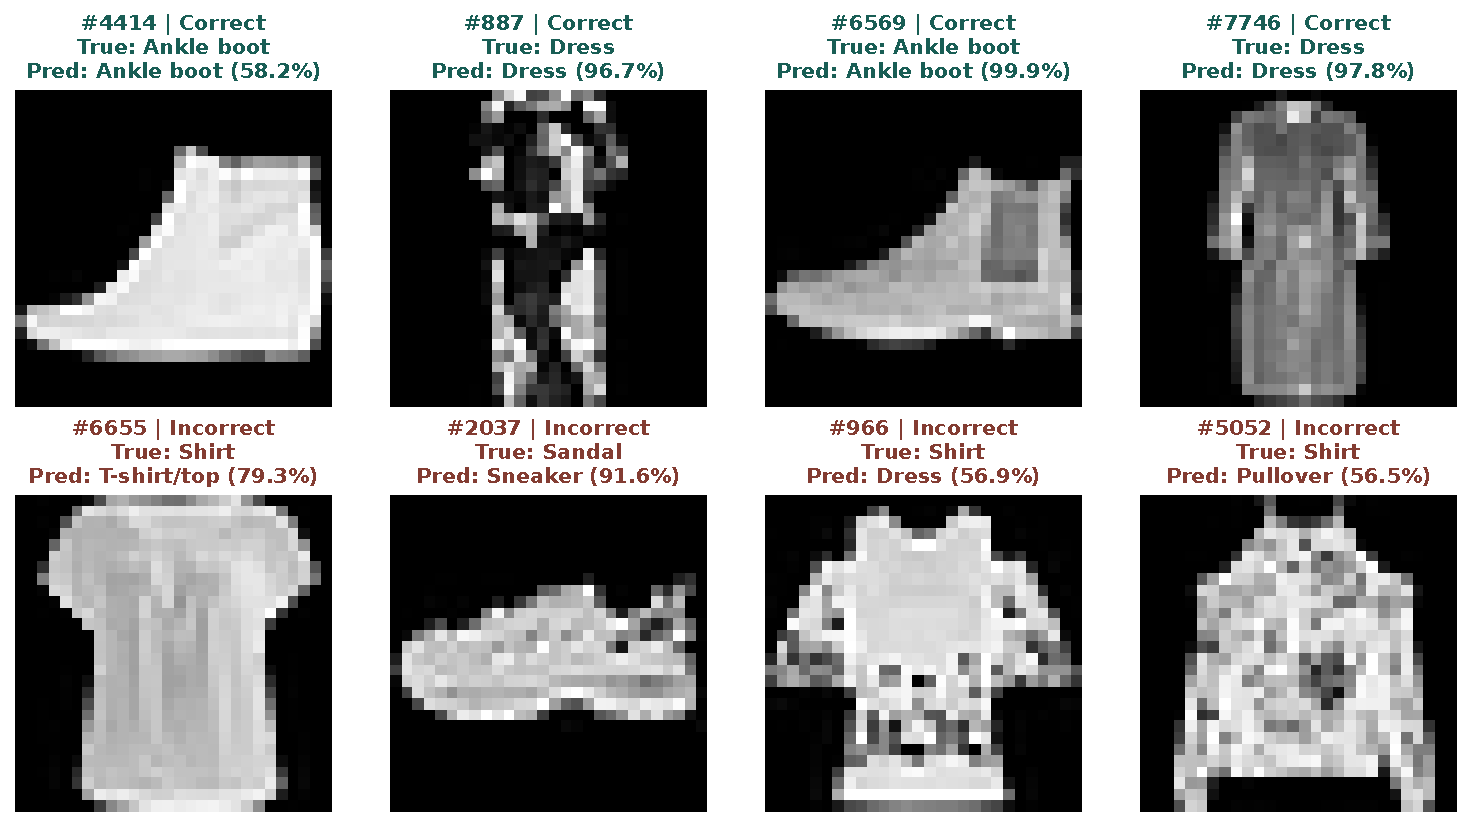
\includegraphics[width=.94\linewidth]{cnn_examples.pdf}
\caption{CNN examples from the official test set, sampled with seed 42.
Indices are zero-based test indices. The percentage is the maximum softmax
score, not a calibrated probability of correctness.}\label{fig:examples}
\end{figure}

Image \#6655 has a short-sleeved outline and is labeled Shirt, but is predicted
as T-shirt/top. Image \#5052 is also Shirt and is predicted as Pullover.
These examples illustrate the upper-body confusion counted in the matrix.
The images alone cannot reveal the model's internal reason for each decision.

The Sandal image \#2037 is predicted as Sneaker with a score of 91.6\%.
In contrast, the correctly classified Ankle boot \#4414 has a score of 58.2\%.
High confidence can accompany an error, and moderate confidence can accompany
a correct prediction. The study does not include a calibration experiment.

\begin{table}[H]\centering
\caption{Paired correctness on the same 10,000 test images.
``Only'' means the named model is correct and the other is wrong.}
\label{tab:paired}
\begin{tabular}{lrrr}\toprule
Compared with CNN & CNN only correct & Other only correct & Both wrong\\\midrule
\tabledata{generated/paired_rows.tex}
\bottomrule\end{tabular}
\end{table}

CNN corrects 566 images that MLP gets wrong, but MLP correctly handles 222 images
that CNN misses. The net difference is the 344-image advantage in Table~\ref{tab:results}.
MLP and LSTM also differ on individual cases: MLP alone is correct on
\MlpOnly{} images and LSTM alone on \LstmOnly{}, producing their two-image net gap.
All five models are wrong on \SharedErrors{} shared images.

These complementary decisions motivate future ensemble experiments, but no
ensemble has been trained or evaluated here. The paired counts describe
agreement and disagreement; they are not an achieved ensemble score.
